% ==============================================================================
% Chapter 4 — UrbEm Tool Upgrade
% ==============================================================================

\chapter{Upgrade of the UrbEm Downscaling Tool}
\label{ch:urbem}

This chapter presents the upgrade of the proxy-development component of
UrbEm. The objective is to construct spatial weights that translate
CAMS sectoral emissions into high-resolution distributions suitable for
urban air-quality modelling. The former workflow provided an operational
set of land-use and activity proxies, but its sector-level structure was
not sufficient for a systematic treatment of point sources, residual
area sources, and sectors whose emissions depend on several distinct
processes. The upgraded methodology therefore distinguishes explicitly
between point-source matching and area-source proxy construction, and it
organises the latter into generic, combined-dataset, and highly
customised approaches. The chapter first establishes this common
methodological framework before presenting the detailed sectoral
implementations.

\section{Proxy construction framework}
\label{sec:framework}

\subsection{Role of proxies in emission downscaling}

Spatial proxies define how emissions reported on a coarse inventory grid
are redistributed to the finer grid required by urban air-quality
modelling. They are therefore not auxiliary cartographic products, but
the main methodological link between an emission inventory and the
spatial pattern imposed on the downscaled emissions. For each pollutant
and sector, the proxy must represent the location of the activity that
generates the emissions as closely as the available evidence allows.

This requirement is particularly important for \cams, because emissions
are reported by GNFR sector and by pollutant, while the spatial drivers
of the processes grouped inside one GNFR sector may differ substantially.
A single land-cover mask can be adequate for a homogeneous residual
source, but it is not sufficient when a sector contains point facilities,
linear infrastructure, population-related activities, industrial land,
livestock processes, or fuel-specific combustion patterns. The proxy
methodology was therefore redesigned around the principle that the
spatialisation method must follow the emission process rather than the
sector label alone.
\begin{figure}[htbp]
  \centering
  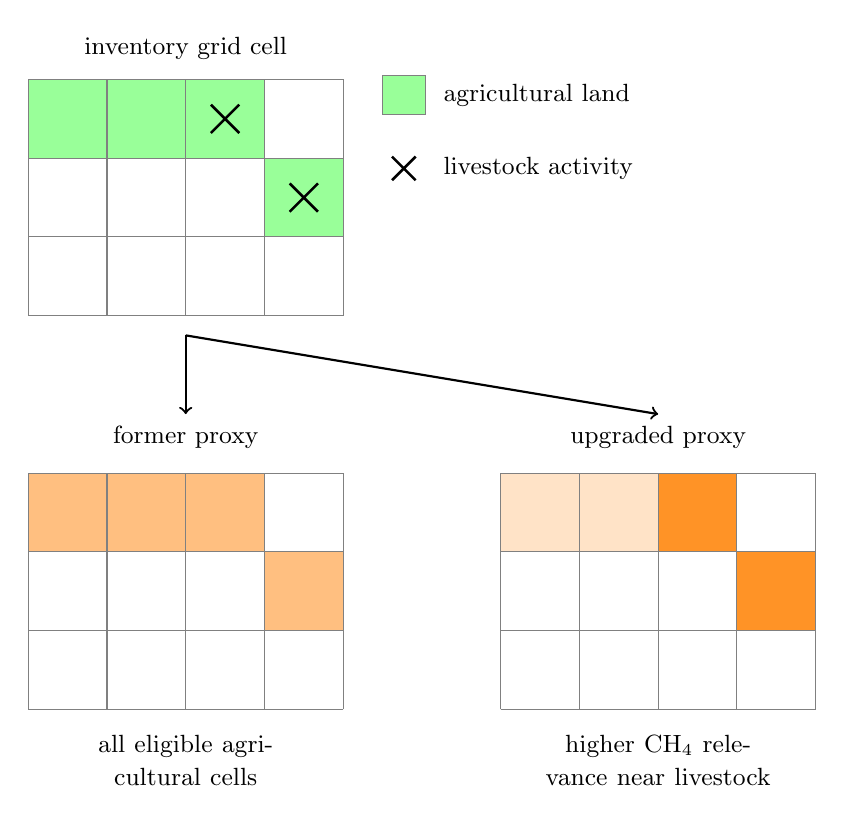
\begin{tikzpicture}[x=1cm, y=1cm]

    %% =========================================================
    %% TOP GRID — bottom-left (0,0), top-right (4,3)
    %% Row 2 (top row):    y = 2 to 3
    %% Row 1 (middle row): y = 1 to 2
    %% Row 0 (bottom row): y = 0 to 1
    %% =========================================================
    \node[align=center] at (2.0, 3.4) {\small inventory grid cell};

    \fill[green!40] (0,2) rectangle (1,3);
    \fill[green!40] (1,2) rectangle (2,3);
    \fill[green!40] (2,2) rectangle (3,3);
    \fill[green!40] (3,1) rectangle (4,2);

    \draw[step=1, line width=0.4pt, color=black!50] (0,0) grid (4,3);

    \foreach \cx/\cy in {2.5/2.5, 3.5/1.5}{
      \draw[line width=0.9pt]
        (\cx-0.18,\cy-0.18)--(\cx+0.18,\cy+0.18)
        (\cx-0.18,\cy+0.18)--(\cx+0.18,\cy-0.18);
    }

    %% LEGEND
    \fill[green!40]   (4.5,2.55) rectangle (5.05,3.05);
    \draw[black!50, line width=0.4pt] (4.5,2.55) rectangle (5.05,3.05);
    \node[anchor=west] at (5.15,2.80) {\small agricultural land};
    \draw[line width=0.9pt]
      (4.62,1.72)--(4.92,2.02)
      (4.62,2.02)--(4.92,1.72);
    \node[anchor=west] at (5.15,1.87) {\small livestock activity};

    %% ARROWS
    \draw[->, line width=0.8pt] (2.0,-0.25) -- (2.0,-1.25);
    \draw[->, line width=0.8pt] (2.0,-0.25) -- (8.0,-1.25);

    %% =========================================================
    %% BOTTOM-LEFT: former proxy
    %% Grid bottom-left (0,-5), top-right (4,-2)
    %% So 3 rows:
    %%   top row    (row2): y = -3 to -2
    %%   middle row (row1): y = -4 to -3
    %%   bottom row (row0): y = -5 to -4
    %%
    %% Pattern mirrors top grid:
    %%   col0,col1,col2 in top row    => y=-3 to -2
    %%   col3           in middle row => y=-4 to -3
    %% =========================================================
    \node[align=center] at (2.0,-1.55) {\small former proxy};

    % TOP ROW fills: y from -3 to -2
    \fill[orange!50] (0,-3) rectangle (1,-2);
    \fill[orange!50] (1,-3) rectangle (2,-2);
    \fill[orange!50] (2,-3) rectangle (3,-2);
    % MIDDLE ROW fill: y from -4 to -3
    \fill[orange!50] (3,-4) rectangle (4,-3);

    \draw[step=1, line width=0.4pt, color=black!50] (0,-5) grid (4,-2);

    \node[align=center, text width=3.0cm] at (2.0,-5.65)
      {\small all eligible agricultural cells};

    %% =========================================================
    %% BOTTOM-RIGHT: upgraded proxy
    %% Grid bottom-left (6,-5), top-right (10,-2)
    %% Same cell positions, differentiated intensity:
    %%   col0,col1 in top row    => LOW  intensity
    %%   col2      in top row    => HIGH intensity
    %%   col3      in middle row => HIGH intensity
    %% =========================================================
    \node[align=center] at (8.0,-1.55) {\small upgraded proxy};

    % TOP ROW
    \fill[orange!22] (6,-3)  rectangle (7,-2);   % col0 low
    \fill[orange!22] (7,-3)  rectangle (8,-2);   % col1 low
    \fill[orange!85] (8,-3)  rectangle (9,-2);   % col2 HIGH
    % MIDDLE ROW
    \fill[orange!85] (9,-4)  rectangle (10,-3);  % col3 HIGH

    \draw[step=1, line width=0.4pt, color=black!50] (6,-5) grid (10,-2);

    \node[align=center, text width=3.5cm] at (8.0,-5.65)
      {\small higher CH$_4$ relevance near livestock};

  \end{tikzpicture}
  \caption{Simplified motivation for process-specific proxy construction.
    A broad agricultural land-cover proxy spreads emissions uniformly over
    all eligible agricultural cells, whereas a process-specific proxy
    amplifies CH$_4$ relevance where livestock activity is present.}
  \label{fig:proxy-process-motivation}
\end{figure}





\subsection{From the former workflow to the upgraded methodology}

The previous UrbEm proxy workflow already provided an operational basis
for downscaling. It constructed a regular modelling grid, prepared
population and land-cover rasters, used selected infrastructure and
facility layers, and produced a set of sectoral proxy rasters. This
former implementation was reviewed sector by sector before the upgrade.
The objective was not to discard the existing methodology, but to
identify which assumptions remained appropriate, which ones were too
generic, and where the treatment of point and area emissions needed to
be separated more explicitly.

The review showed three main limitations. First, several sectors were
represented by broad composite land-cover layers, which made all
pollutants within the same sector inherit the same spatial pattern.
Second, point-like industrial or infrastructure sources were not always
distinguished from residual area sources in a transparent way. Third,
the former procedure was difficult to audit because data preparation,
sector logic, fallback assumptions, and output generation were combined
in a single procedural workflow. These limitations are acceptable for a
first proxy inventory, but they become restrictive when the objective is
to produce sector-specific, pollutant-aware, and reproducible
downscaling weights.

The upgraded methodology therefore separates the proxy problem into
explicit methodological components. Point-source emissions are treated
through a dedicated matching procedure between inventory points and
external facility datasets. Area-source emissions are treated through
sector-specific proxy construction, ranging from simple robust proxies
to multi-dataset and process-specific combinations. This structure makes
the assumptions attached to each sector visible and allows the proxy
outputs to better reflect the heterogeneity of the CAMS emission
structure.

\begin{figure}[htbp]
  \centering
  \setlength{\fboxsep}{5pt}
  \begin{tabular}{c c c c c}
    \fbox{\begin{minipage}{0.17\textwidth}\centering
      Legacy proxy\\workflow
    \end{minipage}} &
    $\longrightarrow$ &
    \fbox{\begin{minipage}{0.20\textwidth}\centering
      Sector-by-sector\\method review
    \end{minipage}} &
    $\longrightarrow$ &
    \fbox{\begin{minipage}{0.24\textwidth}\centering
      Upgraded modular\\proxy methodology
    \end{minipage}} \\
    & & $\downarrow$ & & $\downarrow$ \\
    & &
    \fbox{\begin{minipage}{0.20\textwidth}\centering
      Identification of\\limitations and\\fallbacks
    \end{minipage}} &
    $\longrightarrow$ &
    \fbox{\begin{minipage}{0.24\textwidth}\centering
      Separate treatment of\\point and area\\emissions
    \end{minipage}}
  \end{tabular}
  \caption{Conceptual transition from the former proxy workflow to the upgraded methodology.}
  \label{fig:proxy-old-new-transition}
\end{figure}

\subsection{Point and area emissions in CAMS}

CAMS distinguishes between emissions represented as point sources and
emissions represented as area sources. This distinction is central for
proxy construction. A point source is associated with an explicit
location in the inventory and should, when possible, be linked to a real
facility or installation. An area source represents emissions that are
not resolved as individual facilities in the inventory and must be
redistributed within each CAMS grid cell using spatial indicators.

The methodological consequence is that the same GNFR sector can require
two different proxy treatments. Public power, industry, waste, and
solvent-related activities may contain point-like facilities that should
not be blurred into a generic land-use surface. At the same time, the
same sectors can retain a residual area component that must still be
distributed spatially. Other sectors, such as shipping, fugitive
emissions, off-road transport, agriculture, and residential or commercial
combustion, are dominated by area-source logic or by process-specific
spatial drivers.

\begin{figure}[htbp]
  \centering
  \includegraphics[width=0.98\textwidth]{figures/Proxies/greece_cams_area_share_heatmap.png}
  \caption{Mass share of area and point sources by GNFR sector and pollutant in the CAMS-REG v8.1 inventory for Greece (2019). The full numerical table is given in Appendix~\ref{tab:greece_cams_emis_2019}.}
  \label{fig:gr-area-point-share}
\end{figure}

The point and area contributions are therefore used as a diagnostic step
rather than as a purely descriptive statistic. They indicate whether a
sector should be handled mainly through facility matching, through
area-source proxies, or through a mixed approach. They also help
identify cases where a residual area component is not a separate
physical process, but the part of the gridded inventory that remains
after reported point sources and inventory totals are reconciled.

\begin{figure}[htbp]
  \centering
  \setlength{\fboxsep}{5pt}
  \begin{tabular}{c c c}
    \fbox{\begin{minipage}{0.25\textwidth}\centering
      CAMS emissions\\by sector, pollutant,\\and source type
    \end{minipage}} &
    $\longrightarrow$ &
    \fbox{\begin{minipage}{0.27\textwidth}\centering
      Point-source\\matching to external\\facility records
    \end{minipage}} \\
    $\downarrow$ & & $\downarrow$ \\
    \fbox{\begin{minipage}{0.25\textwidth}\centering
      Sector-specific\\area-source proxy\\construction
    \end{minipage}} &
    $\longrightarrow$ &
    \fbox{\begin{minipage}{0.27\textwidth}\centering
      Normalised proxy\\weights and quality\\control outputs
    \end{minipage}}
  \end{tabular}
  \caption{High-level data flow of the upgraded proxy methodology.}
  \label{fig:proxy-upgraded-dataflow}
\end{figure}

\subsection{Structure of the proxy methodology}

The heatmap in Figure~\ref{fig:gr-area-point-share} shows that the
point--area split is not uniform across sectors or pollutants. Some
sectors are almost entirely area-source in CAMS and can therefore be
handled through area-weight rasters alone. Others contain large point
contributions, or pollutant-dependent mixtures of point and area
emissions, and require a separate facility-matching step before the
residual area component is distributed.

For this reason, the following sections are organised by methodological
need rather than by inventory order. Point-source matching is presented
first because it determines which emissions are assigned to explicit
facilities and should not be redistributed as diffuse area emissions.
Area-source proxies are then described according to increasing
methodological complexity: simple single-layer proxies, combined
multi-dataset proxies, and highly customised process-based approaches.
This structure avoids treating all GNFR sectors as if they required the
same spatial evidence, while keeping the chapter focused on the logic of
proxy construction rather than on a catalogue of outputs.

\subsection{General weight construction}

Although the sectoral methods differ, the area-source part of the
workflow follows a common mathematical logic. Each sector first defines
one or more non-negative spatial indicators on the target reference
grid. These indicators may represent land cover, population, facility
density, transport infrastructure, vessel activity, building-energy
demand, livestock distributions, or other sector-specific drivers. The
indicators are then combined into a raw proxy score and normalised so
that the weights inside each CAMS cell sum to unity.

\subsubsection{Notation}

Throughout this section, the following notation is used:

\begin{table}[h]
  \centering
  \caption{Core notation used for area-source proxy construction.}
  \label{tab:proxy-notation}
  \begin{tabular}{ll}
    \toprule
    Symbol & Meaning \\
    \midrule
    $p$ & pollutant \\
    $s$ & GNFR sector or sectoral component \\
    $m$ & spatial driver, process source, or subsector layer \\
    $j$ & fine-resolution target-grid cell \\
    $C$ & CAMS grid cell containing one or more target-grid cells \\
    $x_{j,m}$ & raw non-negative spatial indicator for driver $m$ in cell $j$ \\
    $\rho_{j,m}$ & scaled relevance of driver $m$ in cell $j$ \\
    $a_{p,m}$ & allocation coefficient for pollutant $p$ and driver $m$ \\
    $S_{j,p}$ & raw combined proxy score for pollutant $p$ in cell $j$ \\
    $w_{j,p}$ & final normalised proxy weight for pollutant $p$ in cell $j$ \\
    \bottomrule
  \end{tabular}
\end{table}

\subsubsection{Spatial indicators and relevance}
\label{sec:relevance-rho}

The raw indicator $x_{j,m}$ expresses the intensity or suitability of
target-grid cell $j$ for spatial driver $m$. Its definition is
sector-specific. For a land-cover proxy, it may be a binary or weighted
class mask. For an infrastructure proxy, it may be the presence or
density of a line or polygon feature. For a process-based proxy, it may
combine several layers before being passed to the final weighting step.

When the magnitude of a raw indicator is not directly comparable across
drivers, it is converted into a dimensionless relevance value. A generic
form is

\begin{equation}
\label{eq:rho-def}
  \rho_{j,m} =
  \begin{cases}
    \dfrac{x_{j,m}}{\displaystyle\max_{j' \in \Omega_m} x_{j',m}},
    & \text{if } \displaystyle\max_{j' \in \Omega_m} x_{j',m} > 0, \\
    0,
    & \text{otherwise,}
  \end{cases}
\end{equation}

where $\Omega_m$ is the spatial support over which driver $m$ is scaled.
Depending on the sector, this support may be a country, a CAMS cell, a
regional mask, or the valid domain of the input layer. The purpose of
this step is not to estimate emissions directly, but to express relative
spatial suitability on a common scale.

\subsubsection{Spatial support and rasterisation}
\label{sec:class-extent}

All area-source indicators are converted to the same target grid before
normalisation. Raster inputs are reprojected and aligned to the
reference grid, while vector inputs are rasterised using the attributes,
buffers, or class memberships defined for the sector. The result is a
set of candidate layers whose cells are spatially comparable and can be
combined without changing the CAMS inventory totals.

This rasterisation step is also where sector-specific spatial support is
defined. Some sectors use broad land-cover classes, others use explicit
infrastructure, facility polygons, vessel-density fields, or building
and population layers. The support therefore differs by sector, but the
final weights always describe how emissions are redistributed within the
CAMS cells retained for the downscaling domain.

\subsubsection{Allocation coefficients}
\label{sec:alpha}

When several drivers contribute to a sector or pollutant, allocation
coefficients determine their relative contribution to the raw proxy
score. These coefficients are denoted by $a_{p,m}$ and may represent
subsector shares, pollutant-specific source fractions, class weights, or
reported allocation factors. For a given pollutant and sectoral
component, they are defined so that the active drivers form a consistent
mixture:

\begin{equation}
  \sum_{m \in \mathcal{M}_{p}} a_{p,m} = 1,
\end{equation}

where $\mathcal{M}_{p}$ is the set of drivers used for pollutant $p$.
If only one spatial driver is used, the corresponding coefficient is
implicitly equal to one.

\subsubsection{Combined score and CAMS-cell normalisation}

The raw proxy score for pollutant $p$ in target-grid cell $j$ is
computed as the weighted sum of the active relevance layers:

\begin{equation}
  S_{j,p} =
  \sum_{m \in \mathcal{M}_{p}}
  a_{p,m} \cdot \rho_{j,m}.
\end{equation}

The final proxy weight is obtained by normalising this score within each
CAMS cell:

\begin{equation}
  w_{j,p} =
  \begin{cases}
    \dfrac{S_{j,p}}
          {\displaystyle\sum_{j' \in C(j)} S_{j',p}},
    & \text{if } \displaystyle\sum_{j' \in C(j)} S_{j',p} > 0, \\
    0,
    & \text{otherwise,}
  \end{cases}
\end{equation}

where $C(j)$ denotes the CAMS cell containing target-grid cell $j$.
This normalisation is the key conservation step: it preserves the CAMS
emission total in each coarse cell while redistributing that total
inside the cell according to the selected proxy surface.

\subsection{Design choices and assumptions}

\paragraph{Conservation within CAMS cells.}
The normalisation is performed within CAMS cells because the downscaling
task is to redistribute the CAMS mass, not to revise the CAMS inventory
itself. The proxy therefore changes the intra-cell spatial pattern but
does not alter the coarse-grid sectoral total.

\paragraph{Sector-specific evidence.}
The workflow does not require every sector to use the same type of
spatial evidence. Simple sectors can use a single robust indicator,
whereas heterogeneous sectors require several drivers and allocation
coefficients. This avoids forcing all emissions into a common land-cover
template when the underlying activities have different spatial controls.

\paragraph{Fallbacks and zero-support cases.}
Some CAMS cells may have no valid proxy support for a given sector and
pollutant. In such cases, the workflow applies the sector-specific
fallback defined for that method, or leaves the cell unallocated when no
scientifically defensible fallback is available. These cases are treated
as quality-control issues because they indicate a mismatch between the
inventory cell and the available spatial evidence.

\paragraph{Allocation coefficients.}
The coefficients used to combine drivers are interpreted as allocation
parameters rather than independent emission estimates. They can be based
on reported sectoral shares, guidebook information, external activity
data, or explicit methodological assumptions. Their role is to distribute
a known CAMS mass across spatial drivers, not to reconstruct the
inventory total.
\section{Point-source matching}
\label{sec:point-source-matching}

\subsection{Motivation}

For sectors with point-source emissions, the downscaling problem is not
limited to deciding how much mass belongs to an inventory point. A more
fundamental difficulty is that CAMS point coordinates do not always
localise the emitting facility precisely. They may fall near the
facility, in the centre of a coarse inventory cell, or at a location that
is spatially displaced from the real industrial installation. Directly
burning these coordinates into the high-resolution proxy grid would
therefore transfer the inventory mass to a location that is not
necessarily the physical source.

The point-source workflow was introduced to correct this limitation as
far as the available facility data allow. Each CAMS point is treated as
an inventory representation of an emitting source. It is then compared
with external facility records that describe real installations. The
objective is not to change the CAMS emission mass, but to identify the
most plausible real-world location to which that mass should be linked.
This distinction is important for later downscaling: the inventory point
preserves traceability to CAMS, while the matched facility provides the
spatial location used to represent the source more realistically.

\subsection{General matching procedure}

The matching workflow starts from the CAMS point-source records selected
for a given GNFR sector, country, year, and representative pollutant. The
representative pollutant is used to rank or filter the CAMS points when
a sector contains many possible records. Candidate facilities are then
assembled from the external dataset most appropriate for the sector. As
far as possible, the external facility sources are selected to remain
consistent with the point-source information reported for the CAMS-REG
inventory compilation \citep{CAMS-REG-v4}. The objective is to avoid
introducing a second, unrelated facility geography while still correcting
the local displacement of the CAMS point coordinates. The datasets are
described in Appendix~\ref{app:datasets}.

For each CAMS point, nearby candidate facilities are screened within a
maximum search distance. This threshold is a hard constraint: a facility
located farther away than the sector-specific maximum distance is not
considered a possible match, even if it has a compatible activity or
pollutant. Candidate pairs that pass this distance screen are then scored
using three criteria. The first criterion is geographical proximity:
shorter distances increase the likelihood that a facility is the correct
match. The second criterion is pollutant consistency: a facility
reporting the same or a closely related pollutant receives a higher score
than a facility with no relevant pollutant information. The third
criterion is activity consistency: facilities belonging to the expected
industrial or sectoral activity class are preferred over facilities from
unrelated activities.

In generic form, the score for a CAMS point--facility pair can be written
as

\begin{equation}
  q =
  \beta_d q_d +
  \beta_p q_p +
  \beta_a q_a ,
\end{equation}

where $q_d$ is the distance score, $q_p$ the pollutant-consistency score,
$q_a$ the activity-consistency score, and the coefficients $\beta_d$,
$\beta_p$, and $\beta_a$ define their relative importance. Distance is
the primary constraint because very distant links are physically
unlikely, while pollutant and activity terms help distinguish between
nearby facilities in industrial clusters.

The same strict and fallback scoring weights are used for all matched
sectors. The sector-specific parameter is the maximum allowed
matching distance, which reflects the expected spatial uncertainty and
facility density of each sector.

\begin{table}[htbp]
  \centering
  \caption{Scoring weights used in the point-source matching procedure.}
  \label{tab:point-source-scoring-weights}
  \begin{tabular}{lccccc}
    \toprule
    Matching stage & $\beta_d$ & $\beta_p$ & $\beta_a$ & Minimum score & Candidate count \\
    \midrule
    Strict & 0.50 & 0.30 & 0.20 & 0.40 & 25 \\
    Fallback & 0.75 & 0.15 & 0.10 & 0.25 & 60 \\
    \bottomrule
  \end{tabular}
\end{table}

The matching is performed in descending order of CAMS point magnitude so
that the largest inventory sources are assigned first. A facility can be
assigned to only one CAMS point, which avoids duplicating the same real
installation across several inventory records. If no sufficiently strong
strict match is found, a fallback stage allows a weaker but still
distance-limited match. This fallback is useful for sectors where the
external facility dataset is incomplete or where facility names and
activity classifications are not fully harmonised across reporting
systems.

\begin{figure}[htbp]
  \centering
  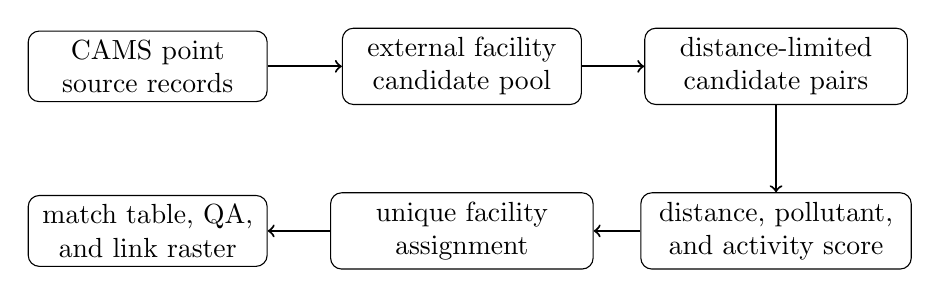
\begin{tikzpicture}[x=0.95cm,y=0.95cm]
    \node[draw, rounded corners, align=center, text width=2.8cm] (cams) at (0,0)
      {CAMS point\\source records};
    \node[draw, rounded corners, align=center, text width=2.8cm] (fac) at (4.2,0)
      {external facility\\candidate pool};
    \node[draw, rounded corners, align=center, text width=3.1cm] (screen) at (8.4,0)
      {distance-limited\\candidate pairs};
    \node[draw, rounded corners, align=center, text width=3.2cm] (score) at (8.4,-2.2)
      {distance, pollutant,\\and activity score};
    \node[draw, rounded corners, align=center, text width=3.1cm] (assign) at (4.2,-2.2)
      {unique facility\\assignment};
    \node[draw, rounded corners, align=center, text width=2.8cm] (out) at (0,-2.2)
      {match table, QA,\\and link raster};

    \draw[->, line width=0.75pt] (cams) -- (fac);
    \draw[->, line width=0.75pt] (fac) -- (screen);
    \draw[->, line width=0.75pt] (screen) -- (score);
    \draw[->, line width=0.75pt] (score) -- (assign);
    \draw[->, line width=0.75pt] (assign) -- (out);
  \end{tikzpicture}
  \caption{General point-source matching workflow. CAMS point records are compared with sector-specific facility candidates, screened by distance, scored using spatial and activity information, and written to diagnostic outputs.}
  \label{fig:point-source-matching-workflow}
\end{figure}

\subsection{Sector-specific facility datasets}

The facility dataset used for matching depends on the sector. This is a
methodological choice rather than a purely technical one: a good match
requires an external dataset whose facilities correspond to the physical
process represented by the CAMS point source. The choice follows the
facility sources reported for CAMS-REG point emissions where possible
\citep{CAMS-REG-v4}, and uses the dataset descriptions given in
Appendix~\ref{app:datasets} for traceability. The matching pollutant is
chosen from the CAMS point-source contribution of each sector, using the
pollutant that best represents the dominant or most diagnostic facility
signal.

\begin{table}[htbp]
  \centering
  \caption{External facility datasets used for point-source matching.}
  \label{tab:point-source-facility-datasets}
  \footnotesize
  \begin{tabular}{p{0.17\textwidth} p{0.27\textwidth} p{0.13\textwidth} p{0.13\textwidth} p{0.20\textwidth}}
    \toprule
    Sector & Facility dataset & Matching pollutant & Maximum distance & Rationale \\
    \midrule
    Public power & JRC Open Power Plants Database & CO & 20 km & CAMS power-point source basis \\
    Industry & E-PRTR and Industrial Emissions reporting & NO$_x$ & 25 km & CAMS industrial point-source basis \\
    Fugitive emissions & E-PRTR and Industrial Emissions reporting & CH$_4$ & 25 km & Energy, mineral, and chemical facilities \\
    Waste & E-PRTR and Urban Waste Water Treatment Directive reporting & CH$_4$ & 12 km & Waste facilities and treatment plants \\
    Solvents & E-PRTR and Industrial Emissions reporting & NMVOC & 10 km & Reported NMVOC-emitting facilities \\
    \bottomrule
  \end{tabular}
\end{table}

For public power, the facility pool is restricted to combustion-related
power plants, excluding non-combustion generation technologies when they
are not relevant for air-pollutant emissions. For industry, the matching
uses industrial reporting facilities and gives preference to activity
classes consistent with industrial combustion and process emissions. For
fugitive emissions, the matching also uses industrial reporting
facilities, but favours energy, mineral, and chemical activities because
these are the most relevant reported facility classes for point-like
fugitive sources. For waste, a combined facility pool is needed because
methane and other waste-sector emissions can originate from reported
waste installations and from waste-water treatment infrastructure. For
solvents, the sector is represented almost exclusively as an area source
in CAMS. However, the Greek CAMS inventory and the industrial reporting
data indicate that many facilities report NMVOC emissions, which
justifies retaining a point-source matching proxy for the facility-like
part of the solvent signal while treating the dominant residual component
through area-source subsector allocation.

\subsection{Two-location representation}

The matching output deliberately preserves both locations: the original
CAMS point and the matched real facility. This is the reason for
constructing a two-layer spatial product. The first layer burns the CAMS
point mass at the original inventory coordinate. The second layer burns
the same linked mass at the matched facility coordinate. Comparing the
two layers makes the spatial displacement visible and documents how much
mass is moved from the inventory point to the real-world installation.

This representation is useful for three reasons. First, it preserves
traceability to the CAMS point source, so the original inventory
information is not lost. Second, it provides the corrected facility-based
location used for high-resolution spatialisation. Third, it supports
quality control, because unusually long links, low scores, or systematic
offsets can be inspected visually before the matched point source is used
in the final downscaling workflow.


\begin{figure}[htbp]
  \centering
  \begin{subfigure}{0.48\textwidth}
    \centering
    \fbox{\begin{minipage}[c][4.0cm][c]{0.92\textwidth}
      \centering
      \includegraphics[width=0.7\textwidth]{figures/Proxies/Capture d'écran 2026-04-28 112834.png}
    \end{minipage}}
    \caption{Public power}
  \end{subfigure}
  \hfill
  \begin{subfigure}{0.48\textwidth}
    \centering
    \fbox{\begin{minipage}[c][4.0cm][c]{0.92\textwidth}
      \centering
      \includegraphics[width=0.7\textwidth]{figures/Proxies/Capture d'écran 2026-04-28 113004.png}
    \end{minipage}}
    \caption{Waste}
  \end{subfigure}
  \caption{Examples of CAMS point-source locations and matched facility locations. These maps are used to verify that the matched facility provides a more plausible physical location than the raw CAMS coordinate. In red the CAMS point location is shown, in blue the matched facility location is shown.}
  \label{fig:point-source-match-examples}
\end{figure}

\subsection{Quality-control outputs}

The point-source procedure produces tabular and spatial diagnostics. The
tabular match output records the CAMS point identifier, matched facility
identifier, coordinates of both locations, distance, score, matched
stage, selected pollutant value, and facility metadata where available.
The quality-control summary reports the number of CAMS points considered,
the number matched, the unmatched count, the coverage rate, and summary
statistics of match distance and score.

These diagnostics are part of the methodology because point-source
matching cannot be treated as a purely automatic operation. A high score
and short distance indicate that the external facility record is a
plausible spatial correction for the CAMS point. A low score or long
distance does not necessarily mean that the match is wrong, but it
signals that the result should be interpreted cautiously. The two-layer
spatial product and the example maps provide the visual counterpart to
the tabular QA, allowing the displacement between inventory coordinates
and facility coordinates to be inspected directly.

\section{Area-source proxy construction}
\label{sec:area-source-proxies}

\subsection{From residual mass to within-cell weights}

After point-source matching, the remaining proxy problem concerns
emissions that are represented by CAMS as area sources. These emissions
do not have a unique facility coordinate. They must therefore be
distributed inside each CAMS cell using spatial information that is
consistent with the activity represented by the sector. The role of an
area-source proxy is to provide this intra-cell distribution while
preserving the CAMS mass in the parent cell.

The area-source workflow follows the conservation principle introduced
in Section~\ref{sec:framework}. For each sector, one or more spatial
indicators are prepared on the common fine grid. These indicators are
converted into a non-negative raw score and then normalised within each
CAMS cell. The proxy therefore changes only the spatial distribution
inside the coarse cell; it does not revise the sectoral or pollutant
total reported by the inventory.

The difficulty is that the appropriate spatial evidence is sector
dependent. Shipping requires marine-traffic and port information. The
residual area component of public power follows a different logic,
because most large emissions are already handled as point sources and
the remaining CAMS area mass represents an inventory residual. Other
sectors require combinations of land use, infrastructure, population,
reported activity, or process-specific drivers. The following area-source
sections are therefore organised by methodological complexity rather than
by GNFR order.

\begin{figure}[htbp]
  \centering
  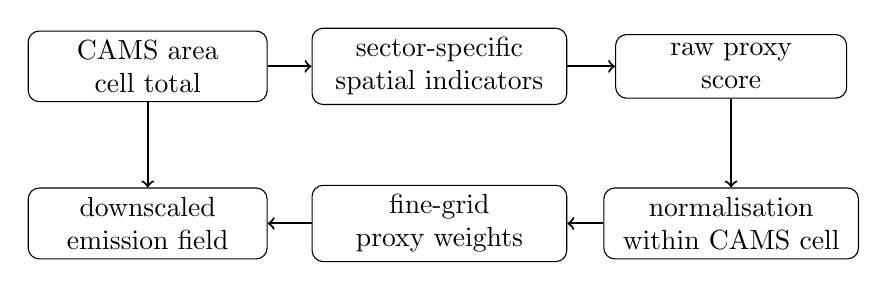
\begin{tikzpicture}[x=0.95cm,y=0.95cm]
    \node[draw, rounded corners, align=center, text width=2.8cm] (cams) at (0,0)
      {CAMS area\\cell total};
    \node[draw, rounded corners, align=center, text width=3.0cm] (drivers) at (3.9,0)
      {sector-specific\\spatial indicators};
    \node[draw, rounded corners, align=center, text width=2.7cm] (score) at (7.8,0)
      {raw proxy\\score};
    \node[draw, rounded corners, align=center, text width=3.0cm] (norm) at (7.8,-2.1)
      {normalisation\\within CAMS cell};
    \node[draw, rounded corners, align=center, text width=3.0cm] (weights) at (3.9,-2.1)
      {fine-grid\\proxy weights};
    \node[draw, rounded corners, align=center, text width=2.8cm] (mass) at (0,-2.1)
      {downscaled\\emission field};

    \draw[->, line width=0.75pt] (cams) -- (drivers);
    \draw[->, line width=0.75pt] (drivers) -- (score);
    \draw[->, line width=0.75pt] (score) -- (norm);
    \draw[->, line width=0.75pt] (norm) -- (weights);
    \draw[->, line width=0.75pt] (weights) -- (mass);
    \draw[->, line width=0.75pt] (cams) -- (mass);
  \end{tikzpicture}
  \caption{General area-source proxy workflow. Sector-specific spatial indicators define a raw score, which is normalised within each CAMS cell before being used to redistribute the corresponding CAMS area-source mass.}
  \label{fig:area-source-workflow}
\end{figure}

\begin{table}[htbp]
  \centering
  \caption{Area-source proxy families used in the upgraded workflow.}
  \label{tab:area-source-families}
  \begin{tabular}{p{0.22\textwidth} p{0.32\textwidth} p{0.22\textwidth} p{0.14\textwidth}}
    \toprule
    Proxy family & When it is used & Examples & Output type \\
    \midrule
    Generic proxy & A small number of robust indicators is sufficient, or the CAMS area mass is a residual component & Shipping; residual public power & Single area-weight layer \\
    Combined-dataset proxy & Several spatial drivers are needed to represent subsectors or activity groups & Waste; industry; fugitive emissions; off-road transport & Sector or pollutant-specific weight layers \\
    Highly customised proxy & The sector requires process-specific allocation or detailed subsector-to-driver mapping & Agriculture; solvents; other combustion & Pollutant or process-weighted layers \\
    \bottomrule
  \end{tabular}
\end{table}

\subsection{Generic area-source proxies}
\label{sec:generic-area-proxies}

Generic proxies are used where a simple spatial logic is scientifically
more defensible than an unnecessarily detailed construction. This does
not mean that the proxy is arbitrary. Rather, the sector either has a
dominant spatial driver that can be represented by a limited set of
harmonised datasets, or the area-source component is a residual mass for
which a complex process decomposition would not be meaningful. In the
current workflow, this category includes shipping and the residual
area-source component of public power. Aviation is kept as a future
generic-proxy candidate because it has not yet been implemented.

\subsubsection{Shipping}
\label{sec:generic-shipping}

Shipping is treated as a single area-source proxy shared by all
pollutants. This choice is appropriate because the main spatial question
is not pollutant-specific process disaggregation, but the recovery of a
plausible maritime and port-related support within the CAMS shipping
cells. The same vessel routes and port environments are relevant for the
allocation of the different shipping pollutants at the resolution used
here.

The proxy combines three spatial indicators. Vessel-density information
provides the main marine-traffic signal and identifies offshore shipping
corridors. Open mapping of port and harbour infrastructure refines the
coastal support. CORINE port-related land cover provides a harmonised
land-cover anchor for port areas. The raw proxy score is defined as a
weighted combination of these three components:

\begin{equation}
  S_{\mathrm{ship}} =
  0.25 D_{\mathrm{vessel}} +
  0.50 D_{\mathrm{port,osm}} +
  0.25 D_{\mathrm{port,clc}},
\end{equation}

where $D_{\mathrm{vessel}}$ is the scaled vessel-density field,
$D_{\mathrm{port,osm}}$ the scaled port-infrastructure support, and
$D_{\mathrm{port,clc}}$ the scaled CORINE port-area support. The larger
weight assigned to the mapped port-infrastructure term reflects its role
as the most explicit high-resolution coastal anchor, while the vessel
density term preserves the offshore traffic structure and the CORINE
term stabilises the port signal in a harmonised European land-cover
framework.

The resulting score is normalised within each CAMS shipping cell. The
final layer is therefore an allocation field rather than an emission
field: it determines how the CAMS shipping total is distributed inside
each parent cell, while preserving the original CAMS mass.

\begin{figure}[htbp]
  \centering
  \begin{subfigure}[b]{0.3\textwidth}
    \centering
    \includegraphics[width=\textwidth, height=4cm, keepaspectratio]{figures/Proxies/shipping_bbox_corine_port_area.png}
    \caption{CORINE port-area}
  \end{subfigure}
  \hfill
  \begin{subfigure}[b]{0.3\textwidth}
    \centering
    \includegraphics[width=\textwidth, height=4cm, keepaspectratio]{figures/Proxies/shipping_bbox_osm_port_area.png}
    \caption{OSM port infrastructure}
  \end{subfigure}
  \hfill
  \begin{subfigure}[b]{0.3\textwidth}
    \centering
    \includegraphics[width=\textwidth, height=4cm, keepaspectratio]{figures/Proxies/shipping_bbox_vessel_density.png}
    \caption{Vessel density}
  \end{subfigure}
  \caption{Visualization of the three spatial proxy components for shipping
    in the Athens area: (a) CORINE land cover (green), (b) OpenStreetMap
    port infrastructure (purple), and (c) vessel density (yellow).}
  \label{fig:athens-shipping-proxies}
\end{figure}

\subsubsection{Residual public power area emissions}
\label{sec:generic-public-power}

Public power is a mixed sector. The main combustion plants are handled
through point-source matching, because they correspond to discrete
facilities. The remaining CAMS area-source component has a different
interpretation. It is not treated as a separate set of known plants, but
as the residual mass left after the inventory reconciles national totals
with explicitly represented point sources. For this reason, a highly
detailed industrial proxy would give a false impression of process
specificity.

The residual area proxy follows the same broad logic used in the CAMS
allocation of unresolved public-power emissions: the residual total is
distributed using population as the main spatial gradient. The upgraded
proxy keeps this population-based logic for consistency with CAMS, but
amplifies the score where the fine grid contains eligible land cover.
Eligible land is defined as CORINE industrial or commercial land and the
equivalent harmonised industrial/built class used on the proxy reference
grid. These pixels are interpreted as more plausible locations for
residual energy-related activity than purely residential or natural
surfaces.

For each fine-grid pixel $j$ inside a CAMS area cell, let
$I_j^{\mathrm{elig}}$ be equal to one on eligible land and zero
elsewhere, and let $P_{01,j}$ be the population field scaled to the
range $[0,1]$ within the same CAMS cell. The raw proxy score is then

\begin{equation}
  S_{\mathrm{pp},j} =
  0.70 \left(I_j^{\mathrm{elig}}\right)^{1 + P_{01,j}}
  + 0.30 P_{01,j},
\end{equation}

where the first term gives priority to eligible land and the second term
retains the population-driven distribution used for the unresolved CAMS
component. This form keeps most of the support on eligible land while
still allowing population to redistribute residual emissions where the
land-cover signal is weak or incomplete.

\begin{figure}[htbp]
  \centering
  \begin{subfigure}[b]{0.3\textwidth}
    \centering
    \includegraphics[width=\textwidth, height=4cm, keepaspectratio]{figures/Proxies/publicpower_bbox_eligible_landcover.png}
    \caption{CORINE eligible land cover}
  \end{subfigure}
  \hfill
  \begin{subfigure}[b]{0.3\textwidth}
    \centering
    \includegraphics[width=\textwidth, height=4cm, keepaspectratio]{figures/Proxies/publicpower_bbox_population_proxy.png}
    \caption{Population proxy}
  \end{subfigure}
  \hfill
  \begin{subfigure}[b]{0.3\textwidth}
    \centering
    \includegraphics[width=\textwidth, height=4cm, keepaspectratio]{figures/Proxies/publicpower_bbox_weights.png}
    \caption{Weights}
  \end{subfigure}
  \caption{Visualization of the two spatial proxy components for PublicPower and the derived weights
    in the Athens area: (a) CORINE land cover (blue), (b) Population (red), and (c) weitghs. Blue lines correspond to CAMS cells }
\label{fig:athens-publicpower-proxies}
\end{figure}



If a CAMS cell contains no eligible land-cover support, the proxy falls
back to population weighting over the valid cell footprint. If population
also provides no usable support, a uniform distribution is used as a last
resort. These fallbacks preserve the CAMS area-source mass while making
the loss of spatial evidence explicit.

\subsubsection{Aviation}
\label{sec:generic-aviation}

Aviation is reserved as a future generic-proxy sector. It has not yet
been implemented in the upgraded workflow and is therefore not used in
the present downscaling chain. When implemented, it should be treated
with the same logic as the other area-source sectors: the proxy should
identify the appropriate airport and flight-activity support, normalise
the resulting score within CAMS cells, and preserve the CAMS sectoral
mass. Until that methodology is implemented and validated, no aviation
area-source proxy is reported here.

\subsection{Combined-dataset area-source proxies}
\label{sec:combined-area-proxies}

The generic proxies described above are sufficient when one spatial
driver dominates the area-source component. Several GNFR sectors,
however, combine source types that are physically distinct but still
reported together in the atmospheric inventory. Waste emissions include
solid-waste handling, wastewater treatment, and residual diffuse sources.
Industrial and fugitive emissions combine many production branches whose
spatial supports differ. Offroad transport includes railways, pipeline
transport, and non-road mobile machinery. For these sectors, a single
land-cover or population layer would obscure the process structure that
is already present in the reported inventory.

The combined-dataset method therefore first builds one spatial indicator
for each interpretable source family. These indicators are then combined
with country- and pollutant-specific allocation coefficients derived from
reported emissions. For a source family $g$, these coefficients are
computed from the reported subgroup emissions as
\begin{equation}
  \alpha_{g,p,c} =
  \frac{\displaystyle\sum_{s \in g} E_{s,p,c}^{\mathrm{rep}}}
       {\displaystyle\sum_{g'}\sum_{s \in g'} E_{s,p,c}^{\mathrm{rep}}},
  \label{eq:combined-alpha-aggregation}
\end{equation}
where $E_{s,p,c}^{\mathrm{rep}}$ is the reported emission of subgroup
$s$, pollutant $p$, and country $c$. This sector-family recombination is
introduced here as part of the upgraded proxy workflow. It builds on the
established foundation of high-resolution emission downscaling, in which
inventory totals are preserved while ancillary spatial data are used to
redistribute emissions within the coarse grid
\citep{UrbEm2021,NAEI2024Spatial}. In the present workflow, the final
step always remains the CAMS-cell normalisation introduced in
Section~\ref{sec:class-extent}; the combined proxy changes only the
within-cell pattern, not the CAMS-cell emission total.

For a sector with source families $g$, the raw score for pollutant $p$ is
written as
\begin{equation}
  S_{p,j} =
  \sum_g \alpha_{g,p,c(j)} P_{g,j},
  \label{eq:combined-sector-score}
\end{equation}
where $P_{g,j}$ is the spatial indicator for family $g$ at fine-grid
cell $j$, and $\alpha_{g,p,c(j)}$ is the reported contribution of that
family to pollutant $p$ in the country $c$ containing cell $j$, computed
as in Equation~\ref{eq:combined-alpha-aggregation}. The final weight is then
\begin{equation}
  W_{p,j \mid C} =
  \frac{S_{p,j}}{\sum_{k \in C} S_{p,k}},
  \qquad j \in C ,
  \label{eq:combined-sector-normalisation}
\end{equation}
with a uniform fallback only when all candidate indicators are zero in a
CAMS cell. This structure keeps the sectoral mass balance explicit while
allowing different pollutants to follow different spatial patterns when
their reported source composition differs.

\subsubsection{Waste}
\label{sec:combined-waste}

Waste is treated as a combined proxy because the sector brings together
solid-waste disposal, wastewater treatment, and residual sources that do
not share the same spatial footprint. This separation is important for
methane and nitrous oxide: wastewater emissions depend on collection,
treatment technology, treatment objectives, and plant size, while
solid-waste emissions are tied to disposal and handling sites
\citep{moore_naturewater2025,Song2024WastewaterNetZero}. The proxy
therefore uses three families: solid waste, wastewater, and residual
diffuse waste.

\begin{table}[htbp]
  \centering
  \caption{Spatial evidence used for the combined waste area-source proxy.}
  \label{tab:waste-spatial-rules}
  \scriptsize
  \begin{tabular}{p{0.18\textwidth} p{0.25\textwidth} p{0.45\textwidth}}
    \toprule
    Family & Spatial weighting & Retained evidence \\
    \midrule
    Solid waste &
    $1.00$ dump-site support, $0.35$ industrial or commercial support, and $0.50$ mapped solid-waste support. &
    CORINE 132 dump sites; CORINE 121 industrial or commercial units; OSM landfill, waste\_disposal, recycling, and other solid-waste-related mapped polygons or buffered points. \\
    Wastewater &
    $0.45$ agglomeration cover, $0.35$ treatment-plant support, $0.35$ population, $0.25$ imperviousness, and $0.08$ industrial context. &
    Reported wastewater agglomeration polygons; reported treatment-plant points buffered around facilities; population density; impervious surface; CORINE 131 mineral extraction, 132 dump sites, and 133 construction sites as industrial context. \\
    Residual diffuse waste &
    $0.50$ population, $0.35$ rural settlement support, and $0.15$ imperviousness. &
    Population density; rural settlement classes from the settlement model; impervious surface as a settlement support indicator. \\
    \bottomrule
  \end{tabular}
\end{table}

Each family proxy is constructed from the spatial evidence listed in
Table~\ref{tab:waste-spatial-rules} after quantile-based scaling of the
input indicators. Treatment plants are buffered and slightly smoothed so
that wastewater treatment is represented as a local treatment zone rather
than as a single fine-grid cell.

\begin{table}[htbp]
  \centering
  \caption{Waste source families used for pollutant-specific allocation coefficients.\tablefootnote{Reported source-group definitions follow the EMEP/EEA air pollutant emission inventory guidebook \citep{EMEP_EEA}.}}
  \label{tab:waste-alpha-groups}
  \scriptsize
  \begin{tabular}{p{0.18\textwidth} p{0.18\textwidth} p{0.30\textwidth} p{0.26\textwidth}}
    \toprule
    Proxy family & Reported codes & Reported source groups represented & Interpretation in the area proxy \\
    \midrule
    Solid waste &
    5A; 5B1; 5B2 &
    Solid-waste disposal on land and biological treatment of waste. &
    Emissions are allocated to dump sites, waste-management land, recycling or disposal features, and related mapped waste facilities. \\
    Wastewater &
    5D1; 5D2; 5D3 &
    Domestic wastewater handling, industrial wastewater handling, and other wastewater-related releases. &
    Emissions are allocated to wastewater agglomerations, treatment plants, and the serviced urban population context. \\
    Residual diffuse waste &
    5C2; 5E &
    Small combustion of waste, other waste handling, and waste activities not represented by the two facility-oriented families. &
    Emissions are allocated more diffusely using population, rural settlement, and impervious-surface indicators. \\
    \bottomrule
  \end{tabular}
\end{table}

Waste incineration codes 5C1a and 5C1b are excluded from the area-source
family recombination because they are not treated as diffuse residual
waste in this proxy.

For each pollutant, the three waste families are combined as
\begin{equation}
  S_{\mathrm{waste},p,j} =
  \alpha_{\mathrm{solid},p,c(j)} P_{\mathrm{solid},j}
  + \alpha_{\mathrm{ww},p,c(j)} P_{\mathrm{ww},j}
  + \alpha_{\mathrm{res},p,c(j)} P_{\mathrm{res},j}.
  \label{eq:waste-composite}
\end{equation}
If one family has no local support in a given fine cell, its coefficient
is not allowed to create emissions there. The active family coefficients
are renormalised locally before the CAMS-cell normalisation in
Equation~\ref{eq:combined-sector-normalisation}. This avoids suppressing
the proxy when, for example, wastewater facilities are absent in a rural
cell but the residual waste component remains plausible.


The detailed visual workflow for the waste proxy construction is given
in Appendix~\ref{app:ceip-weights}, 
\subsubsection{Industry}
\label{sec:combined-industry}
Industrial area emissions are represented through four source families, each targeting
a distinct production environment: refineries and petroleum handling \textit{G1}, general
manufacturing combustion and residual industry \textit{G2}, mineral products \textit{G3}, and
chemicals and metals \textit{G4}.  The four-group decomposition is introduced here because the pollutant
composition and spatial footprint of these activities differ substantially. Refinery
stacks and petroleum storage are geographically concentrated and emit a profile
dominated by $\text{SO}_x$ and VOCs, whereas general manufacturing combustion produces a
broader $\text{NO}_x$ and PM mixture distributed across generic industrial zones. Mineral
production --- cement, lime, glass, and quarrying --- generates process PM and $\text{SO}_x$
from sites that are spatially distinct from general industry, and is therefore supported
by CORINE class~131 (mineral extraction sites) combined with OSM quarry and works
features. Chemical manufacturing and primary metal production are strong point-like
sources of $\text{SO}_x$, heavy metals, and reactive nitrogen whose spatial concentration
differs markedly from both general manufacturing and mineral sites
\citep{EMEP_EEA, CAMS-REG-v4}. Treating all four families under a single generic
industrial proxy would misallocate these contrasted emission profiles across the grid.
Each group is assigned country- and pollutant-specific coefficients
$\alpha_{g,p,c}$ derived from CEIP-reported subgroup emissions following
Eq.~\ref{eq:combined-alpha-aggregation}. G1 through G4 represent the residual
area mass, which for petroleum handling likely corresponds to smaller storage and
distribution infrastructure not individually reported at high spatial precision
\citep{Crippa2016, CAMS-REG-v4}.
For each industrial group $g$, the raw spatial indicator is constructed from a
group-specific OSM component, a group-specific CORINE component, and a weak population
fallback:
%
\begin{equation}
  p_{g,j} =
  \begin{cases}
    w_{g,\mathrm{sec}}
    \bigl(
      w_{g,\mathrm{osm}}\, \mathcal{Z}(O_{g,j})
      + w_{g,\mathrm{clc}}\, \mathcal{Z}(C_{g,j})
    \bigr)
    + w_{g,\mathrm{pop}}\, P_j
    & \text{if } O_{g,j} + C_{g,j} > 0, \\[6pt]
    P_j
    & \text{otherwise,}
  \end{cases}
  \label{eq:industry-group-proxy}
\end{equation}
%
where $O_{g,j}$ and $C_{g,j}$ are respectively the OSM coverage fraction and the
CORINE score for group $g$ at pixel $j$, $P_j$ is the population proxy raster,
$\mathcal{Z}(\cdot)$ is a standardisation operator that places both inputs on a
comparable scale, and $w_{g,\mathrm{sec}} = 1 - w_{g,\mathrm{pop}}$. When no
industrial evidence is present in a pixel, the proxy falls back entirely to population,
consistent with the residual mass allocation used in \mbox{CAMS-REG-ANT} itself. The
resulting $p_{g,j}$ is subsequently normalised within each CAMS cell to obtain the
final redistribution weights.

The OSM component concentrates emissions around explicitly mapped industrial
infrastructure, while the CORINE component provides areal support where OSM tagging is
incomplete. The population term is not interpreted as a direct driver of industrial
activity; it serves only as a spatial fallback for diffuse residual emissions whose
facility evidence is locally absent. Group-specific weights are summarised in
Table~\ref{tab:industry-spatial-rules}.

For G1, the spatial indicator combines OSM features tagged as oil or fuel works,
refineries, and fuel storage tanks ($w_{\mathrm{osm}} = 0.82$) with CORINE class~121
($w_{\mathrm{clc}} = 0.15$) and a minimal population fallback
($w_{\mathrm{pop}} = 0.03$). Refineries are strongly point-like facilities; the
population term is retained only to cover residual storage and distribution
infrastructure not individually mapped. For G2, generic OSM industrial landuse,
factory and warehouse buildings, and fossil-fuel power plant features
($w_{\mathrm{osm}} = 0.55$) are combined with CORINE~121 ($w_{\mathrm{clc}} = 0.35$)
and a population fallback ($w_{\mathrm{pop}} = 0.10$); this group acts as a catch-all
for the heterogeneous residual of manufacturing combustion and ancillary industrial
processes (NFR~2D--2L), where diffuse emissions justify a larger population share. For
G3, OSM quarry, mineshaft, and mineral works features ($w_{\mathrm{osm}} = 0.65$) are
combined with CORINE~131 mineral extraction sites ($w_{\mathrm{clc}} = 0.30$) and a
small population fallback ($w_{\mathrm{pop}} = 0.05$); quarrying and mineral
processing are predominantly rural activities with low residential co-location. For G4,
OSM chemical, pharmaceutical, petrochemical, and metal works features
($w_{\mathrm{osm}} = 0.75$) are combined with CORINE~121 ($w_{\mathrm{clc}} = 0.20$)
and a minimal population fallback ($w_{\mathrm{pop}} = 0.05$); heavy industry and
primary metal production are strongly concentrated and poorly correlated with
population density.

\begin{table}[htbp]
  \centering
  \caption{Spatial evidence and weights used for the industry area-source proxy.
           $w_{\mathrm{sec}} = 1 - w_{\mathrm{pop}}$ in all cases.}
  \label{tab:industry-spatial-rules}
  \scriptsize
  \begin{tabular}{p{0.18\textwidth} p{0.24\textwidth} p{0.46\textwidth}}
    \toprule
    Group & Weights & Retained spatial evidence \\
    \midrule
    G1 --- Refineries and petroleum handling &
    $w_{\mathrm{osm}}=0.82$,\newline
    $w_{\mathrm{clc}}=0.15$,\newline
    $w_{\mathrm{pop}}=0.03$ &
    OSM: petroleum works, refineries, oil and fuel industrial sites, storage tanks,
    depots.\newline
    CORINE: 121 industrial or commercial units. \\[4pt]
    G2 --- Manufacturing combustion and residual industry &
    $w_{\mathrm{osm}}=0.55$,\newline
    $w_{\mathrm{clc}}=0.35$,\newline
    $w_{\mathrm{pop}}=0.10$ &
    OSM: industrial land, factories, warehouses, works, manufacturing, textile, food,
    sawmill, engineering, machine-shop, gas, oil, and biomass plant features.\newline
    CORINE: 121 industrial or commercial units. \\[4pt]
    G3 --- Mineral products &
    $w_{\mathrm{osm}}=0.65$,\newline
    $w_{\mathrm{clc}}=0.30$,\newline
    $w_{\mathrm{pop}}=0.05$ &
    OSM: quarries, mineshafts, cement, lime, glass, ceramic, and brick works.\newline
    CORINE: 131 mineral extraction sites. \\[4pt]
    G4 --- Chemicals and metals &
    $w_{\mathrm{osm}}=0.75$,\newline
    $w_{\mathrm{clc}}=0.20$,\newline
    $w_{\mathrm{pop}}=0.05$ &
    OSM: chemical, pharmaceutical, fertiliser, petrochemical, plastic, steel, iron,
    aluminium, copper, zinc, metal, foundry, smelting, and rolling-mill features.\newline
    CORINE: 121 industrial or commercial units. \\
    \bottomrule
  \end{tabular}
\end{table}


\begin{table}[htbp]
  \centering
  \caption{Industry source groups used for pollutant-specific allocation coefficients.}
  \label{tab:industry-alpha-groups}
  \scriptsize
  \begin{tabular}{p{0.18\textwidth} p{0.22\textwidth} p{0.28\textwidth} p{0.24\textwidth}}
    \toprule
    Proxy group & Reported codes & Reported source groups represented & Interpretation in the area proxy \\
    \midrule
    Refineries and petroleum handling &
    1A1b; 1A1c; 1B1b; 1B2a5; 1B2a6; 1B2b5; 2C1b &
    Petroleum refining, petroleum storage, fuel depots, and related refinery or petroleum handling sources. &
    Allocates petroleum-related process and handling emissions to refinery, storage, depot, and industrial land supports. \\
    Manufacturing combustion and residual industry &
    1A2a--1A2f; 1A2gvii; 1A2gviii; 2D1; 2D2; 2D3a; 2D3b; 2G; 2H1--2H3; 2I--2L &
    Manufacturing combustion, machinery, food, textiles, wood, paper, product use, and residual industrial activities. &
    Allocates residual industrial combustion and diffuse manufacturing-process emissions to general industrial supports. \\
    Mineral products &
    2A1; 2A2; 2A3; 2A4a--2A4d; 2A5a--2A5c; 2A6 &
    Cement, lime, glass, ceramics, quarrying, construction products, and other mineral processes. &
    Allocates process emissions toward mineral extraction, cement, construction, and industrial land. \\
    Chemicals and metals &
    2B1--2B7; 2B8a--2B8f; 2B9a; 2B9b; 2B10a; 2B10b; 2C1--2C6; 2C7a--2C7d &
    Chemical industry, pharmaceutical and fertiliser production, iron and steel, non-ferrous metals, and foundries. &
    Allocates emissions to chemical and metal-production supports. \\
    \bottomrule
  \end{tabular}
\end{table}


\begin{figure}[htbp]
  \centering
  \fbox{\parbox{0.88\textwidth}{\centering
  Placeholder for the industry proxy figure: panels for refineries and
  petroleum handling, manufacturing combustion and residual industry,
  mineral products, chemicals and metals, and final selected-pollutant
  weight.}}
  \caption{Suggested diagnostic figure for the combined industry proxy.
  The figure should show the difference between petroleum, manufacturing,
  mineral, and chemical or metal supports before
  pollutant-specific recombination.}
  \label{fig:industry-combined-proxy-placeholder}
\end{figure}

\subsubsection{Fugitive emissions}
\label{sec:combined-fugitive}

Fugitive emissions are highly process-dependent. Methane releases from
fuel extraction, handling, and transmission can be concentrated around
energy infrastructure, while some downstream and residual activities are
more diffuse. Satellite-based studies confirm that fossil-fuel methane
emissions are spatially heterogeneous and often dominated by production
basins, coal activities, and high-emitting infrastructure
\citep{Lu2023FuelMethane}. The fugitive proxy therefore separates coal
and solid fuels, oil transport and upstream handling, storage or refining
and distribution, and gas flaring or residual fuel losses before
pollutant-specific recombination.

\begin{table}[htbp]
  \centering
  \caption{Spatial evidence used for the fugitive-emissions area-source proxy.}
  \label{tab:fugitive-spatial-rules}
  \scriptsize
  \begin{tabular}{p{0.20\textwidth} p{0.23\textwidth} p{0.45\textwidth}}
    \toprule
    Group & Spatial weighting & Retained evidence \\
    \midrule
    Coal and solid fuels &
    $\lambda_{\mathrm{OSM}}=0.60$, $\lambda_{\mathrm{CLC}}=0.40$; final group score $0.80$ sector signal and $0.20$ population. &
    Coal, mine, quarry, and industrial-land features; CORINE 131 mineral extraction and 121 industrial or commercial units. \\
    Oil transport and upstream handling &
    $\lambda_{\mathrm{OSM}}=0.60$, $\lambda_{\mathrm{CLC}}=0.40$; final group score $0.80$ sector signal and $0.20$ population. &
    Pipeline, port, depot, and oil-industrial features; CORINE 123 port areas and 121 industrial or commercial units. \\
    Storage, refining, and distribution &
    $\lambda_{\mathrm{OSM}}=0.60$, $\lambda_{\mathrm{CLC}}=0.40$; final group score $0.80$ sector signal and $0.20$ population. &
    Refineries, storage tanks, fuel storage, depots, and fuel-service features; CORINE 121 industrial or commercial units and 122 road or rail networks and associated land. \\
    Gas flaring and residual losses &
    $\lambda_{\mathrm{OSM}}=0.60$, $\lambda_{\mathrm{CLC}}=0.40$; final group score $0.80$ sector signal and $0.20$ population. &
    Flares, chimneys, power plants, generators, substations, gas-industrial features, and gas-resource features; CORINE 121 industrial or commercial units and 131 mineral extraction. \\
    \bottomrule
  \end{tabular}
\end{table}

The spatial construction mirrors the industry workflow, but the retained
features are selected to represent fuel-related activities:
\begin{equation}
  P_{g,j}^{\mathrm{fug}} =
  \mathcal{N}
  \left(
    \lambda_{g,\mathrm{osm}} O_{g,j}^{\mathrm{fug}}
    + \lambda_{g,\mathrm{clc}} C_{g,j}^{\mathrm{fug}}
    + \lambda_{g,\mathrm{pop}} P_{\mathrm{pop},j}
  \right).
  \label{eq:fugitive-group-proxy}
\end{equation}
The population component is kept weak and is used only where a reported
group cannot be represented fully by mapped infrastructure.

\begin{table}[htbp]
  \centering
  \caption{Fugitive-emission groups used for pollutant-specific allocation coefficients.}
  \label{tab:fugitive-alpha-groups}
  \scriptsize
  \begin{tabular}{p{0.19\textwidth} p{0.18\textwidth} p{0.31\textwidth} p{0.24\textwidth}}
    \toprule
    Proxy group & Reported codes & Reported source groups represented & Interpretation in the area proxy \\
    \midrule
    Coal and solid fuels &
    1B1A; 1B1B; 1B1C &
    Coal mining, post-mining handling, and solid-fuel losses. &
    Allocates emissions toward extraction land and coal-related industrial features. \\
    Oil transport and upstream handling &
    1B2AI &
    Oil transport, upstream oil handling, port transfer, and depot activity. &
    Allocates emissions to pipeline, port, depot, and oil-industrial supports. \\
    Storage, refining, and distribution &
    1B2AIV; 1B2AV &
    Petroleum storage, refineries, distribution depots, and fuel handling. &
    Allocates emissions to storage tanks, refineries, depots, and transport-associated land. \\
    Gas flaring and residual losses &
    1B2B; 1B2C; 1B2D &
    Gas flaring, venting, residual fuel losses, and associated energy infrastructure. &
    Allocates emissions to flares, chimneys, energy facilities, gas infrastructure, and industrial land. \\
    \bottomrule
  \end{tabular}
\end{table}

The combined fugitive score is
\begin{equation}
  S_{\mathrm{fug},p,j} =
  \sum_g
  \alpha_{g,p,c(j)} P_{g,j}^{\mathrm{fug}} .
  \label{eq:fugitive-composite}
\end{equation}
This is especially relevant for CH$_4$, for which oil, gas, and coal
families can dominate the reported mass, but the same framework is kept
for all pollutants in order to preserve a consistent multiband output.

\begin{figure}[htbp]
  \centering
  \fbox{\parbox{0.88\textwidth}{\centering
  Placeholder for the fugitive-emissions proxy figure: panels for coal
  and solid fuels, oil transport and upstream handling, storage or
  refining and distribution, gas flaring or residual losses, and final
  CH$_4$ weight.}}
  \caption{Suggested diagnostic figure for the fugitive-emissions proxy.
  The CH$_4$ panel is the most important diagnostic because methane is the
  dominant pollutant for many fuel-related fugitive sources.}
  \label{fig:fugitive-combined-proxy-placeholder}
\end{figure}

\subsubsection{Offroad transport}
\label{sec:combined-offroad}

The offroad transport sector is constructed from three separate activity
families: railways, pipeline transport, and non-road mobile machinery.
These families are combined because they are reported together in the
inventory category, but their spatial evidence is fundamentally
different. Rail emissions follow railway infrastructure, pipeline
transport follows pipeline corridors and associated facilities, and
non-road machinery is linked to land uses where mobile equipment is
expected to operate. National spatial-emission methodologies commonly use
such infrastructure and land-use information to allocate non-road and
rail-related emissions when direct activity data are unavailable
\citep{NAEI2024Spatial}.

\begin{table}[htbp]
  \centering
  \caption{Spatial evidence used for the offroad transport area-source proxy.}
  \label{tab:offroad-spatial-rules}
  \scriptsize
  \begin{tabular}{p{0.20\textwidth} p{0.25\textwidth} p{0.43\textwidth}}
    \toprule
    Family & Spatial weighting & Retained evidence \\
    \midrule
    Rail transport &
    Railway-line coverage buffered by 150 m; activity share given by $\alpha_{\mathrm{rail},p,c}$. &
    Active railway lines and railway land-use polygons; inactive or unsuitable railway values such as abandoned, disused, razed, and proposed are excluded. \\
    Pipeline transport &
    Pipeline coverage buffered by 75 m; the present setup uses the line proxy directly. If a facility raster is supplied, the blend is $0.80$ line signal and $0.20$ facility signal. &
    Pipeline lines, pipeline-related areas, and associated pipeline facilities where available. \\
    Non-road mobile machinery &
    $0.50$ agricultural support and $0.35$ industrial support before pollutant-specific recombination. &
    CORINE agricultural classes 211--213 and 241--243, optional permanent crops 221--223, industrial and extraction classes 121, 131, 133, and optional port areas 123. \\
    \bottomrule
  \end{tabular}
\end{table}

The rail and pipeline components are built as buffered infrastructure
coverage scores, while the non-road component is a CORINE-only activity
support. The pollutant-specific score is
\begin{equation}
  S_{\mathrm{off},p,j} =
  \alpha_{\mathrm{rail},p,c(j)} Z_{\mathrm{rail},j}
  + \alpha_{\mathrm{pipe},p,c(j)} Z_{\mathrm{pipe},j}
  + \alpha_{\mathrm{nonroad},p,c(j)} P_{\mathrm{nonroad},j}.
  \label{eq:offroad-composite}
\end{equation}
Here, $Z_{\mathrm{rail}}$ and $Z_{\mathrm{pipe}}$ are standardised
infrastructure-coverage scores, and $P_{\mathrm{nonroad}}$ is the
land-cover machinery proxy. The coefficients are pollutant-specific
because the relative contribution of railway engines, pipeline transport,
and non-road machinery differs between pollutants.

\begin{table}[htbp]
  \centering
  \caption{Offroad transport source families used for pollutant-specific allocation coefficients.}
  \label{tab:offroad-alpha-groups}
  \scriptsize
  \begin{tabular}{p{0.20\textwidth} p{0.16\textwidth} p{0.32\textwidth} p{0.24\textwidth}}
    \toprule
    Proxy family & Reported code & Reported source groups represented & Interpretation in the area proxy \\
    \midrule
    Rail transport &
    1A3c &
    Railway transport emissions. &
    Allocates emissions to active railway corridors and railway land. \\
    Pipeline transport &
    1A3ei &
    Pipeline transport and compressor or distribution-related pipeline activity. &
    Allocates emissions to pipeline corridors and related mapped infrastructure. \\
    Non-road mobile machinery &
    1A3eii &
    Mobile machinery used outside road transport, including agricultural, industrial, construction, and service equipment. &
    Allocates emissions to land-cover classes where machinery use is plausible. \\
    \bottomrule
  \end{tabular}
\end{table}

After construction of $S_{\mathrm{off},p,j}$, the score is normalised
within each CAMS cell with Equation~\ref{eq:combined-sector-normalisation}.
The output is pollutant-specific because each band receives the reported
rail, pipeline, and non-road shares for that pollutant.

\begin{figure}[htbp]
  \centering
  \fbox{\parbox{0.88\textwidth}{\centering
  Placeholder for the offroad proxy figure: panels for rail coverage,
  pipeline coverage, non-road land-cover support, and the final selected
  pollutant weight.}}
  \caption{Suggested diagnostic figure for the offroad proxy. The figure
  should make clear that rail and pipeline families follow infrastructure
  corridors, while non-road machinery is represented through land-cover
  support.}
  \label{fig:offroad-combined-proxy-placeholder}
\end{figure}



% Further sectoral proxy blocks can be added here, for example:
% \section{Public Power}
\label{sec:publicpower}

\subsection{Motivation}

At first sight, Public Power appears to be the sector for which no real
downscaling is needed. Public electricity and heat production is a classical
\emph{point-source} activity: emissions originate from plants whose locations
are physically defined. One would therefore expect the inventory coordinates to
be sufficient, so that no additional spatial redistribution would be needed.

Inspection of the CAMS-REG-ANT GNFR~A inventory and of the CAMS methodology
showed that this assumption is only partly true. Two observations justify a
dedicated proxy:
\begin{itemize}
  \item GNFR~A contains both point sources and area sources, so the sector is
        not represented exclusively by explicit stacks.
  \item Even where CAMS labels a source as a point, the reported coordinates
        are not always precise enough for high-resolution allocation.
\end{itemize}

The area component is not an accident of the file structure. In the CAMS
compilation logic, national totals for public electricity and heat production
are compared against the emissions that can be assigned to known plants. The
remaining difference is retained as residual \emph{area-source} mass and is
distributed spatially using population as a first-order allocator
\cite{CAMS_glob_ant_61}. Public Power is therefore a mixed spatial system: it
is dominated by point sources, but it also contains a residual area component
produced by the inventory construction itself.

The upgraded workflow therefore creates two proxy layers:
\begin{itemize}
  \item a point-source localisation layer for the explicit plant component;
  \item an area-source downscaling layer for the residual surface emissions.
\end{itemize}

\subsection{Point-source proxy: localisation of combustion units}

\paragraph{Rationale.}
For true power-plant emissions, no classical downscaling is required in the
sense of spreading emissions over land-cover classes. What is required is a
better localisation layer than the raw CAMS point coordinates. The upgraded
method therefore treats point-source Public Power as a \emph{localisation}
problem: identify the pixels that plausibly host thermal generation units and
use that support to anchor the point component.

The point layer is built from a European open power-plant register described
in Appendix~\ref{app:powerplant_register}. Only combustion-based public-power
units are retained, while hydro and other non-combustion generation types are
excluded because the objective is to represent stack-related emissions.

\paragraph{Proxy definition.}
Let $g$ denote a pixel on the national CORINE reference grid and let
$U_{\mathrm{comb}}$ be the set of retained combustion units. The point proxy is
a binary support raster:
\begin{equation}
  \mu_{g}^{\mathrm{pp,point}} =
  \begin{cases}
    1, & \exists\,u \in U_{\mathrm{comb}} \text{ with } x_u \in g,\\
    0, & \text{otherwise},
  \end{cases}
\end{equation}
where $x_u$ is the location of unit $u$. In other words, a reference-grid
pixel receives value one if at least one retained combustion unit falls inside
it. The binary choice is deliberate: it expresses plant presence without
letting a few large multi-unit sites dominate purely through registry
granularity.

\paragraph{Interpretation.}
This layer should not be read as a full reconstruction of plant-level
emissions. It is a spatial support surface answering a narrower question:
where are public-power point emissions most plausibly located at fine
resolution?

\subsection{Area-source proxy: residual CAMS mass distributed over suitable land}

\paragraph{Rationale.}
The existence of CAMS GNFR~A area emissions means that a second proxy is
necessary. Here a genuine downscaling problem does arise, because the residual
public-power mass must be redistributed from coarse CAMS area cells to fine
pixels. The chosen proxy follows the logic already embedded in the CAMS
methodology: if the residual originates from the gap between national totals
and explicitly reported plants, and CAMS distributes that gap using
population, then a population-based area proxy is methodologically coherent
rather than arbitrary.

The area layer combines three ingredients: the CAMS area-source geometry, a
CORINE-based suitability mask, and a gridded population field that controls
the within-cell intensity gradient.

\paragraph{Proxy definition.}
Let $k$ denote a CAMS GNFR~A area cell and let $g \in k$ index fine pixels
inside that cell on the reference grid. Define the CORINE eligibility flag
\begin{equation}
  I_g^{\mathrm{CLC}} =
  \begin{cases}
    1, & \mathrm{CLC}_g \in \mathcal{C}_{\mathrm{pp}},\\
    0, & \text{otherwise},
  \end{cases}
\end{equation}
and let $P_g$ be the LandScan population value resampled to pixel $g$. The raw
within-cell score is
\begin{equation}
  \mu_{g,k}^{\mathrm{pp,area}} =
  I_g^{\mathrm{CLC}} \cdot \max(P_g, P_0)^{\beta},
\end{equation}
where $P_g$ is the population value in pixel $g$. The
normalised within-cell weight is then
\begin{equation}
  w_{g,k}^{\mathrm{pp,area}} =
  \frac{\mu_{g,k}^{\mathrm{pp,area}}}
       {\displaystyle\sum_{g' \in k} \mu_{g',k}^{\mathrm{pp,area}}},
\end{equation}
so that the weights inside each CAMS area cell sum to unity.

This separates two roles clearly: land cover defines \emph{where} residual
public-power emissions may be placed, while population defines \emph{how much}
of the CAMS cell total each eligible pixel receives.

\paragraph{Fallback logic.}
Some CAMS area cells contain no pixels belonging to the selected CORINE
classes. In that case, the implementation falls back first to
population-only weighting over all valid pixels in the cell and, if necessary,
to a uniform distribution over the valid cell footprint. This avoids losing
area-source mass purely because the high-resolution land-cover layer does not
intersect the coarse CAMS rectangle in the expected way.

\subsection{How the point and area layers are used together}

GNFR~A is represented by two complementary spatial products because the
inventory itself contains two geometries. For area sources, pollutant $p$ from
CAMS source $s$ is redistributed within its parent CAMS cell using
\begin{equation}
  e_{g,s,p}^{\mathrm{area}} = E_{s,p} \, w_{g,s}^{\mathrm{pp,area}}.
\end{equation}
For point sources, the role of the proxy is different: emissions are not
spread across land-cover classes but constrained to pixels for which
\(\mu_{g}^{\mathrm{pp,point}} > 0\), that is, pixels hosting at least one
retained combustion unit.

Public Power is therefore not treated as a single undifferentiated proxy.
Instead, the method does two things at once: it \emph{relocates} the point
component more credibly, and it \emph{downscales} the residual area component
in a way consistent with the CAMS methodology.

\subsection{Limitations and forward path}

The main limitations are straightforward. The point layer is a binary plant
presence raster rather than a one-to-one reconciliation of individual plant
records. The plant register is also incomplete, so omission and location error
remain possible. Finally, the area layer assumes that residual public-power
emissions follow population once restricted to suitable land. That assumption
is defensible because it mirrors the inventory logic, but it does not resolve
the internal diversity of diffuse public-power activities.

% \input{chapters/04A_proxies/04A2_OffRoad_proxies}
% \input{chapters/04A_proxies/04A4_Waste_proxies}